\chapter{Test}

Es wurden im späteren Verlauf Änderungen durchgeführt. Es wurde ein Branch angelegt in dem die alle Test vorhanden sind \href{https://github.com/lorenz1702/Spy-Game/tree/UnitTestBranch}{TestBranch}.

Menschen sind die Architekten der digitalen Welt, aber sie sind auch fehlbar. Jeder, der Software entwickelt, weiß, dass Fehler unvermeidlich sind. Und diese Fehler können teuer sein - in Geld, Zeit und sogar in Bezug auf Vertrauen und Nerven. Die Kosten eines Fehlers steigen mit der Zeit seiner Existenz. Selbst wenn ein Fehler sofort erkannt und behoben wird, hinterlässt er dennoch seine Spuren.

In Deutschland sind Softwaretests gesetzlich vorgeschrieben, und das aus gutem Grund. Das Nichttesten wird als "grob fahrlässig" angesehen. Tests helfen dabei, gewollte Funktionen von zufälligen Features zu unterscheiden. Legacy Code, also Code ohne Tests, kann zu einem schwerwiegenden Problem werden.

Einige Entwickler setzen Tests als Werkzeug in ihrer täglichen Arbeit ein. Testgetriebene Entwicklung ist eine Methode, bei der Tests vor dem eigentlichen Code geschrieben werden. Dies stellt sicher, dass jede Funktionalität von Tests begleitet wird und somit die Qualität und Stabilität der Software gewährleistet wird. Letztendlich sind Tests ein unverzichtbarer Bestandteil des Entwicklungsprozesses, der dazu beiträgt, dass Software fehlerfrei und vertrauenswürdig ist.

% Welche Funktion haben tests
\begin{comment}
\section{Leistungstest}
% was sind Leistungstests
Leistungstests sind entscheidend, um die Leistungsfähigkeit eines Systems unter realen Bedingungen zu bewerten. Beim Start eines vollständigen Systems werden möglicherweise zusätzliche Sensoren verwendet, um wichtige Kenngrößen zu erfassen. Eine echte oder Referenzumgebung mit einer realen Datenbank und Hardware ist unerlässlich, um realitätsnahe Ergebnisse zu erzielen.

Durch die Einbeziehung zahlreicher simulierter Klienten oder Benutzer können parallele Bedienungsdurchführungen mit den Mitteln des Benutzers simuliert werden. Das Hauptziel besteht darin, echte Lastbedingungen zu erzeugen und wichtige Kenngrößen zu ermitteln, um die Leistung des Systems zu bewerten.

Es ist wichtig zu betonen, dass Leistungstests nicht darauf abzielen, die Korrektheit des Systems zu überprüfen. Ihr Fokus liegt vielmehr auf der Messung der Reaktionsfähigkeit, Skalierbarkeit und Stabilität unter verschiedenen Belastungsbedingungen, um sicherzustellen, dass das System den Anforderungen unter Last gerecht wird.
\section{Integrations Test}
%was sind intergations Test 
Integrationstests sind eine wichtige Art von Tests, die darauf abzielen, das reibungslose Zusammenspiel der verschiedenen Komponenten eines Systems sicherzustellen. Dabei werden nur die relevanten Teile des Systems gestartet, während nicht zu testende Teile durch Stellvertreter ersetzt werden. Dies ermöglicht es, isoliert auf die Interaktionen zwischen den Komponenten zu fokussieren.

Die Durchführung der Integrationstests erfolgt in der Regel mithilfe eines Testframeworks, das Methodenaufrufe zwischen den verschiedenen Komponenten simuliert. Hierbei werden die Interaktionen der Systemteile untereinander überprüft, um sicherzustellen, dass sie gemäß den Spezifikationen zusammenarbeiten.

Das Hauptziel von Integrationstests besteht darin, das Zusammenspiel der Komponenten sicherzustellen und sicherzustellen, dass sie ordnungsgemäß miteinander kommunizieren können. Dabei liegt der Fokus auf der Integration und Interaktion der Komponenten, während Einzelheiten der einzelnen Komponenten nicht im Vordergrund stehen. Integrationstests überprüfen also nicht die inneren Details der Komponenten, sondern vielmehr deren Zusammenwirken im Gesamtsystem.


\end{comment}
\section{Unit Test}
%Was sind Unit test? Welche funktionen haben sie ?
Unit-Tests, auch bekannt als Komponententests, sind eine grundlegende Form von Tests in der Softwareentwicklung, die darauf abzielen, die korrekte Implementierung einer einzelnen Komponente, oft einer Methode oder Funktion, sicherzustellen. Bei Unit-Tests wird nur der relevante Teil des Systems gestartet, während alle anderen Teile durch Stellvertreter ersetzt werden. Dies ermöglicht es, isoliert auf die Funktionalität der Komponente zu fokussieren.

Die Durchführung von Unit-Tests erfolgt in der Regel mithilfe eines Testframeworks, das Methodenaufrufe der zu testenden Komponente simuliert. Dabei werden die Rückgabewerte der Methoden überprüft, um sicherzustellen, dass sie den erwarteten Ergebnissen entsprechen.

Das Hauptziel von Unit-Tests besteht darin, die korrekte Implementierung der einzelnen Komponente sicherzustellen. Dabei liegt der Fokus auf der Prüfung der Funktionalität und des Verhaltens der Komponente unter verschiedenen Bedingungen. Unit-Tests testen jedoch nicht das Zusammenspiel zwischen verschiedenen Komponenten oder die Performance des Systems, sondern konzentrieren sich ausschließlich auf die Funktionalität der einzelnen Einheiten.

Hier wurden jetzt 10 Unit Test verwendet um die GameReository Klasse zu test. Zuvor wurde der zu testende Code nicht vollständig überprüft. Von den 10 Unit tests fallen vier durch. Damit haben die Unit tests ihr Ziel erfüllt die Korrektheit der Implementierung zu überprüfen\href{https://github.com/lorenz1702/Spy-Game/commit/9142232564a086007dc335c17d2dc9fa30309729}.

\begin{lstlisting}[language=Kotlin, caption={Test and the wrong code}, label={lst:1}]
    @Test
    fun createUsers() {
        // Arrange
        val users = listOf(
            Player(1, "Player 1"),
            Player(2, "Player 2"),
            Spy(3, "Spy 1")
        )
        val game = InMemoryGameRepository()
        game.createUsers(1,2)

        assertEquals(users, game.getAllUser())

override fun createUsers(numberOfSpies: Int, numberOfPlayers: Int) {
    for (i in 1..numberOfSpies) {
        -createSpy(i)
        +this.addSpy(createSpy(i))
        }
    for (i in 1..numberOfPlayers) {
        -createPlayer(i)
        +this.addPlayer(createPlayer(i))
    }
}

}
    
\end{lstlisting}

In diesem Beispiel hat der Unit-Test einen entscheidenden Sinn gezeigt. Er ist durchgefallen, und dadurch wurde entdeckt, dass die Liste keine Benutzer enthielt, weil vergessen wurde, die Benutzer in der Liste zu speichern. Dieser Fehler wurde aufgedeckt, weil der Test die erwartete Funktionalität mit der tatsächlichen Implementierung verglich. Dies verdeutlicht die Bedeutung von Unit-Tests, um sicherzustellen, dass jede Komponente einer Software gemäß den Anforderungen funktioniert.\ref{lst:1}



\section{ATRIP-Regeln}
Fünf Regeln für gute Unit Tests
\subsection*{Automatic - Eigenständig}

Automatic bedeutet, dass Tests eigenständig ablaufen müssen, ohne dass manuelle Eingriffe erforderlich sind. Dies bedeutet, dass keine Dialoge weggeklickt werden müssen und keine manuellen Werteeingaben erfolgen dürfen. Die Tests müssen in der Lage sein, ihre Ergebnisse selbst zu überprüfen. Dabei ist für jeden Test nur das Ergebnis "bestanden" oder "nicht bestanden" zulässig. Wenn ein Test nicht besteht, wird dies als "gebrochen" bezeichnet. Durch die Einhaltung dieser Regeln wird eine Testdurchführung ohne zusätzliches Wissen ermöglicht, was wiederum die Automatisierung der Tests erleichtert.\href{https://github.com/lorenz1702/Spy-Game/commit/9142232564a086007dc335c17d2dc9fa30309729}{Commit-Hash} Alle Tests sind automatisch ausführbar. 


\subsection*{Thorough - Gründlich}
Tests sollten nicht nur oberflächlich sein, sondern durchdringend und gründlich, um sicherzustellen, dass alle relevanten Aspekte einer Anwendung ordnungsgemäß funktionieren. Das Konzept von "though" in Bezug auf Tests bedeutet, dass sie alles Notwendige abdecken, um die Anforderungen und Rahmenbedingungen der Anwendung zu erfüllen. Dies wird in diesem Commit erfüllt in dem die Core Funktionen gestestet werden die Missions Kritisch sind.\href{https://github.com/lorenz1702/Spy-Game/commit/b0692bf0d1c65c3f4af85381358f92dc94f1eeca}{Commit-Hash}

\subsection*{Repeatable - Wiederholbar}
%Alle Tests sind wiederholbar. 
Der Test der diese Funktion getestet hatte war nicht gut wiederholbar der unterschiedliche Ergebnisse geliefert hat, da die Funktion einen Zufall enthällt. Jetzt werden die Rahmenbedingungen getestet um sicherzustellen das die Funktion korrekt abläuft.
\begin{lstlisting}[language=Kotlin, caption={Repetable}, label={lst:2}]
override fun DisplayOneRole() {

        if (users.isEmpty()) {
            println("No more users left.")
            return
        }

        val randomIndex = (0 until users.size).random()
        val randomUser = users.removeAt(randomIndex)

        println("${randomUser.username}:")
        randomUser.displayRole()
        if (randomUser is Player) {
                println("Word: ${Game.getWord()?.name}")  // Print the word if the user is a player and not a spy
        }
}
@Test
fun displayOneRole() {
    // Arrange
    gameRepository = mock()
    impCoreFunktions = ImpCoreFunktions(gameRepository)
    val player1 = Player(1, "Player 1")
    val player2 = Player(2, "Player 2")
    val spy1 = Spy(3, "Spy 1")
    val usersList = mutableListOf<User>(player1, player2, spy1)

    impCoreFunktions.users = usersList.toMutableList()

    // Mocking gameRepository to return a word
    `when`(gameRepository.getWord()).thenReturn(Word(1,"TestWord"))

    // Act
    impCoreFunktions.DisplayOneRole()

    // Assert
    assertEquals(usersList.size - 1, impCoreFunktions.users.size)
}
\end{lstlisting}
In dem wird getestet, ob die Größe der Liste um eins verkleinert wurde.\ref{lst:2}

\subsection*{Independent - Unabhängig voneinander}
Tests müssen jederzeit in beliebiger Zusammenstellung und Reihenfolge funktionsfähig sein. Das bedeutet, dass keine impliziten Abhängigkeiten zwischen den Tests bestehen sollten, wie beispielsweise persistente Datenstrukturen wie Datenbanken oder Dateisysteme. Idealerweise sollte jeder Test genau einen Aspekt der Komponente überprüfen. Im Falle eines Fehlers sollte ein Test fehlschlagen, nicht hunderte, und die Ursache für den Testausfall sollte möglichst direkt ableitbar sein. Dies ermöglicht eine effiziente Fehlersuche und -behebung während des Testprozesses.

Hier wird die StartGame()-Methode gemockt, sodass, falls die StartGame()-Methode einen Fehler hat, nur der Test für die StartGame()-Methode abbricht und nicht auch die anderen. Siehe \ref{lst:3}.
\begin{lstlisting}[language=Kotlin, caption={Independent}, label={lst:3}]
fun displayOneRole() {
    // Arrange
    gameRepository = mock()
    impCoreFunktions = ImpCoreFunktions(gameRepository)
    val player1 = Player(1, "Player 1")
    val player2 = Player(2, "Player 2")
    val spy1 = Spy(3, "Spy 1")
    val usersList = mutableListOf<User>(player1, player2, spy1)

    impCoreFunktions.users = usersList.toMutableList()

    // Mocking gameRepository to return a word
    `when`(gameRepository.getWord()).thenReturn(Word(1,"TestWord"))

    // Act
    impCoreFunktions.DisplayOneRole()
    }
\end{lstlisting}
\subsection*{Profressional - Mit Sorgfalt hergestellt}
Test Code ist ebenso produktionsrelevant wie der eigentliche Code. Dennoch unterliegt Test Code selbst nicht automatischen Tests. Fehler in Tests können schwerwiegend sein und kostenintensive Reparaturen nach sich ziehen. Daher sollte Test Code so klar und verständlich wie möglich sein. Es ist nicht ratsam, die Anzahl der Tests rein quantitativ zu erhöhen, ohne deren Qualität zu berücksichtigen. Ebenso sind Tests für irrelevante Aspekte nicht zielführend und sollten vermieden werden.
\begin{lstlisting}[language=Kotlin, caption={Profressional}, label={lst:4}]
@Test
fun endGame() {

    // Arrange
    gameRepository = mock()
    impCoreFunktions = ImpCoreFunktions(gameRepository)
    val player1 = Player(1, "Player 1")
    val player2 = Player(2, "Player 2")
    val spy1 = Spy(3, "Spy 1")
    val usersList = mutableListOf<User>(player1, player2, spy1)

    impCoreFunktions.users = usersList.toMutableList()

    // Act
    impCoreFunktions.EndGame()

    // Assert
    verify(gameRepository, times(1)).userdisplaythereRole()
}
\end{lstlisting}

Lesbarkeit und Verständlichkeit: Der Test ist gut strukturiert und dokumentiert, was er überprüft und welche Interaktionen erwartet werden. Dadurch ist der Test leicht verständlich und kann von anderen Entwicklern einfach nachvollzogen werden \href{lst:4}.
\section{Mocked Test}
%Was sind gemockede Tests und welche funktionen haben sie 
Mock-Objekte, oft einfach als "Mocks" bezeichnet, sind einfache Stellvertreter für "echte" Objekte in der Softwareentwicklung. Sie dienen dazu, Abhängigkeiten während eines Tests zu ersetzen, ähnlich wie ein Licht-Double in der Filmindustrie nur die beleuchtungsrelevanten Eigenschaften eines echten Stars besitzt.

Die Verwendung von Mocks ermöglicht die Isolation von Klassen während des Tests. Um eine Klasse isoliert testen zu können, müssen ihre Abhängigkeiten durch Mock-Objekte ersetzt werden. Diese Mocks bieten eine Minimalumsetzung der notwendigen Funktionalität, auch bekannt als Fakes, die "gut genug" für den Testeinsatz sind.

Obwohl selbst programmierte Mocks zeitaufwendig sein können, lohnt sich der Einsatz von Mock-Tools, die speziell für diesen Zweck entwickelt wurden. Mocks müssen für ihren jeweiligen Einsatzzweck "trainiert" werden und durchlaufen dabei drei Phasen: das Einlernen (Training-Phase), das Abspielen (Einsatz-Phase) und die Überprüfung (Verifikation-Phase). Ein Beispiel dafür findet man hier \ref{lst:2} und in diesem \href{https://github.com/lorenz1702/Spy-Game/commit/b0692bf0d1c65c3f4af85381358f92dc94f1eeca}{Commit-Hash}

%Example
Die verify-Methode in Mockito wird verwendet, um sicherzustellen, dass bestimmte Interaktionen mit Mock-Objekten während des Tests aufgetreten sind. Sie ermöglicht es, zu überprüfen, ob bestimmte Methoden eines Mock-Objekts aufgerufen wurden und mit welchen Argumenten.

Im Kontext des zuvor bereitgestellten Unit-Tests wird verify verwendet, um sicherzustellen, dass die StartGame-Funktion der ImpCoreFunktions-Klasse bestimmte Methoden des GameRepository-Interfaces mit den erwarteten Argumenten aufruft. Zum Beispiel:

\begin{lstlisting}[language=Kotlin, label={lst:5}]

verify(gameRepository).createUsers(numberOfSpys, numberOfUsers - numberOfSpys)
\end{lstlisting}
Diese Zeile überprüft, ob die createUsers-Methode des GameRepository-Mockobjekts mit den angegebenen Argumenten (numberOfSpys und numberOfUsers - numberOfSpys) während der Ausführung der StartGame-Funktion aufgerufen wird.

Zusammenfassend ist verify eine Mockito-Methode, die verwendet wird, um Methodenaufrufe auf Mock-Objekten zu überprüfen, um sicherzustellen, dass das zu testende System sich wie erwartet verhält.

Durch die Verwendung von Mock-Objekten und der verify-Methode von Mockito wird die Interaktion mit dem gameRepository überprüft, ohne tatsächliche Änderungen am GameRepository vorzunehmen. Dies stellt sicher, dass der Test unabhängig von externen Ressourcen ist und jederzeit wiederholbar ist. Darüber hinaus ist der Test leicht verständlich, da er klar angibt, welches Verhalten überprüft wird und welche Interaktionen erwartet werden. Somit trägt dieser Test zur Stabilität und Qualität des Codes bei, indem er sicherstellt, dass die EndGame-Funktion wie erwartet funktioniert.
\section{Code Coverage}
Testabdeckung, auch bekannt als Code Coverage, ist ein Maß dafür, wie viel von Ihrem Quellcode während der Ausführung Ihrer Tests abgedeckt wird. Es gibt verschiedene Arten von Testabdeckung, von denen die beiden gängigsten Line Coverage und Branch Coverage sind.

Die Line Coverage misst, welche Zeilen Ihres Codes von Ihren Tests durchlaufen werden. Eine Zeile gilt als abgedeckt, wenn sie während der Testausführung mindestens einmal ausgeführt wird.

Die Branch Coverage hingegen betrachtet die Verzweigungen oder Entscheidungspunkte in Ihrem Code. Sie misst, wie viele Verzweigungspunkte durch Ihre Tests abgedeckt werden, indem sie sowohl den Wahrheitswert true als auch false erreichen.

Es ist wichtig zu beachten, dass die Testabdeckung als Bezugspunkt dient und nicht als alleiniges Maß für die Qualität Ihrer Tests betrachtet werden sollte. Eine hohe Testabdeckung deutet zwar darauf hin, dass ein großer Teil Ihres Codes getestet wurde, sagt jedoch nichts über die Qualität der Tests oder die tatsächliche Fehlerabdeckung aus. Dennoch kann die Testabdeckung ein nützliches Werkzeug sein, um Bereiche Ihres Codes zu identifizieren, die möglicherweise zusätzliche Tests erfordern.
\begin{figure}[h]
    \centering
    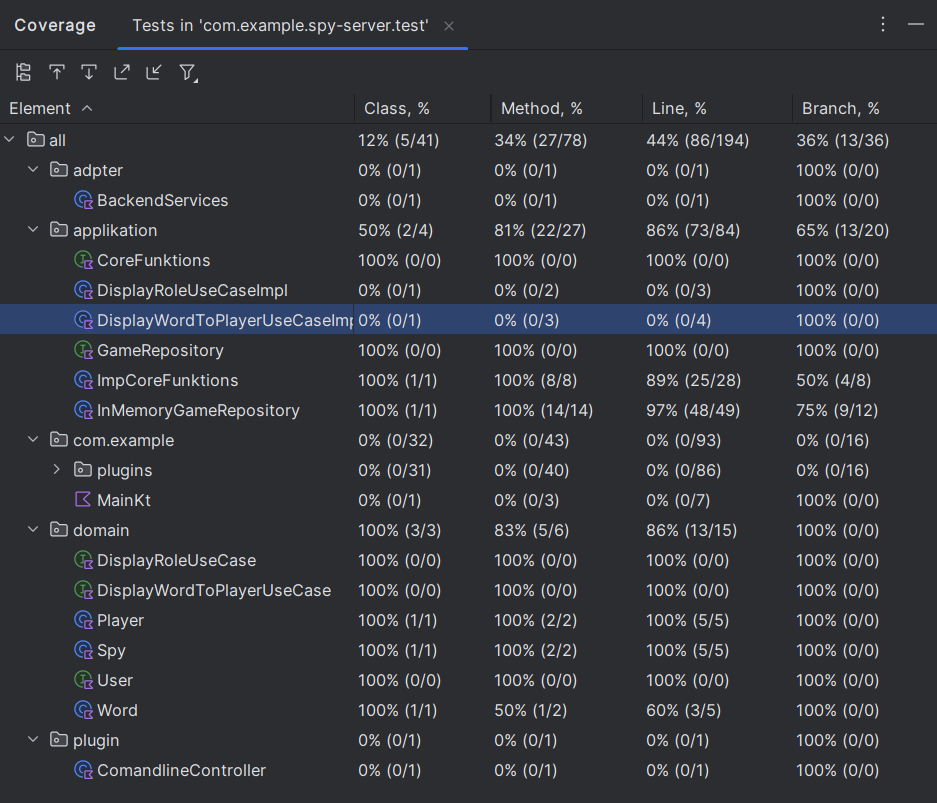
\includegraphics[width=10cm]{images/image.png}
    \caption{Code Coverage}
    \label{fig:12}
\end{figure}
Die Testabdeckung zeigt, dass derzeit nur ein kleiner Teil des Codes durch Tests abgedeckt ist.

Insgesamt beträgt die Testabdeckung für alle Klassen 12,2\%. Das bedeutet, dass nur etwa 12,2\% des Codes durch Tests getestet werden. Dies ist ein niedriger Wert und deutet darauf hin, dass viele Teile des Codes nicht ausreichend getestet wurden.

Eine detaillierte Analyse der Testabdeckung zeigt, dass einige Pakete und Klassen besser abgedeckt sind als andere:

\begin{itemize}
    \item Das Paket "applikation" hat eine Testabdeckung von 50\% für Klassen, 81,5\% für Methoden, 65\% für Verzweigungen und 86,9\% für Zeilen. Dies deutet darauf hin, dass dieses Paket besser getestet ist als andere, aber es gibt immer noch Bereiche, die verbessert werden könnten.
    
    \item Das Paket "domain" hat eine höhere Testabdeckung, mit 100\% für Klassen, 83,3\% für Methoden und 86,7\% für Verzweigungen. Dies deutet darauf hin, dass dieses Paket gründlicher getestet wurde und weniger ungetestete Bereiche aufweist.
    
    \item Die anderen Pakete wie "adpter", "com.example" und "com.example.plugins" haben eine Testabdeckung von 0\%, was darauf hindeutet, dass sie überhaupt nicht getestet wurden.
\end{itemize}

Insgesamt zeigt die Analyse der Testabdeckung, dass es noch viel Raum für Verbesserungen gibt. Eine höhere Testabdeckung ist wichtig, um die Zuverlässigkeit und Qualität des Codes sicherzustellen und potenzielle Fehler zu identifizieren. Es ist ratsam, die Testabdeckung schrittweise zu verbessern, indem mehr Tests hinzugefügt und ungetestete Bereiche abgedeckt werden.

Hier wurde die Code Coverage durch geführt \href{https://github.com/lorenz1702/Spy-Game/commit/735b2712fbacca8f45f3a4fd820081cb8efeea14}{Commit-Hash}
